\subsection{Diagramme de classe}

	Le diagramme présent sur la figure \ref{diagrammeClasse} permet de représenter les différentes activités et classes utilisées dans l'application.
	
\begin{sidewaysfigure}
	\includegraphics[scale=0.6]{img/diagrammeClasse.png}
	\caption{Diagramme de classe}
	\label{diagrammeClasse}
\end{sidewaysfigure}

\subsection{Diagramme de navigation}

	Le diagramme présent sur la figure \ref{diagrammeNavigation} permet de représenter les transitions entre chaque page de l'application. 
	
	\begin{figure}[!h]
		\begin{center}	
	   		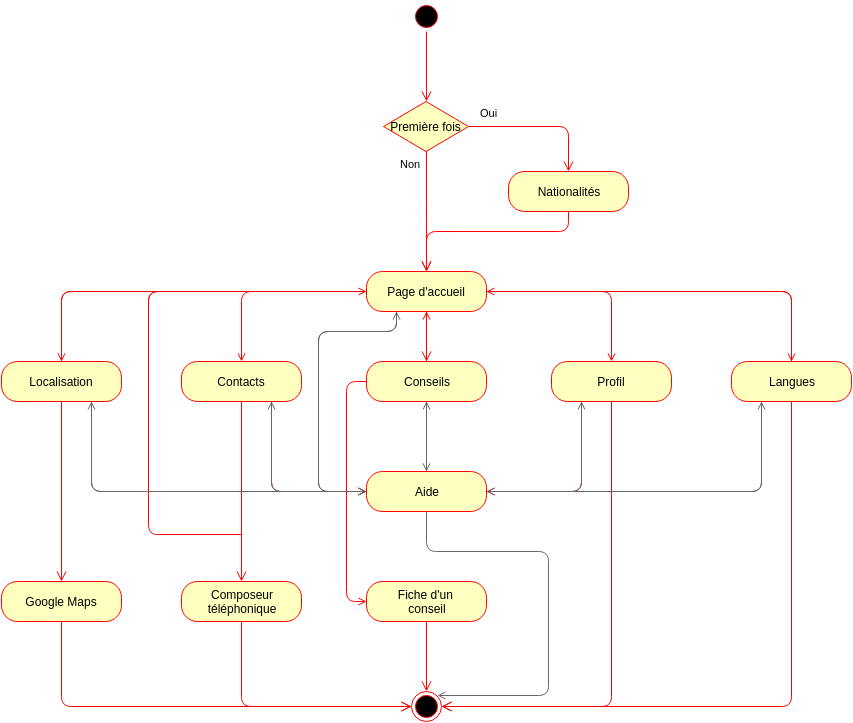
\includegraphics[scale=0.6]{img/navigation.png}
	   		\caption{Diagramme de navigation}
	   		\label{diagrammeNavigation} 	
		\end{center}
	\end{figure}

\newpage